% This is a simple sample document.  For more complicated documents take a look in the exercise tab. Note that everything that comes after a % symbol is treated as comment and ignored when the code is compiled.

\documentclass[9pt, twocolumn]{article} % \documentclass{} is the first command in any LaTeX code.  It is used to define what kind of document you are creating such as an article or a book, and begins the document preamble

\usepackage{amsmath} % \usepackage is a command that allows you to add functionality to your LaTeX code

\usepackage{amsfonts}

\usepackage{amsmath}

\usepackage{graphicx}

\usepackage[T1]{fontenc}
% \usepackage{tgbonum}
\usepackage{lmodern}

\usepackage{titlesec}
\titleformat{\section}{\large\bfseries}{\thesection}{1em}{}
\titleformat{\subsection}{\normalsize\bfseries}{\thesubsection}{1em}{}
\usepackage[font=footnotesize]{caption}

\usepackage[
  backend=biber,
  style=alphabetic,
  sorting=ynt
]{biblatex}
\addbibresource{reffs.bib} %Import the bibliography file

\title{Compte rendu : Bruits à variation spatialle en temps réel} % Sets article title
\author{Arthur Chateauneuf} % Sets authors name
\date{\today} % Sets date for date compiled

% The preamble ends with the command \begin{document}
\begin{document} % All begin commands must be paired with an end command somewhere
\fontsize{9pt}{10pt}\selectfont

\onecolumn
\maketitle % creates title using information in preamble (title, author, date)
\tableofcontents
\twocolumn

\clearpage

%======================= INTRODUCTION =======================%
\section{Introduction}

\subsection{Contexte du stage}

\subsection{Présentation du sujet et des problématiques}

\subsubsection{Processus Stochastique}

\subsubsection{Variation Spatialle}

\subsubsection{Temps réel: utilisations et implications}

\subsubsection{Parrallélisation}
\subsubsection{Complexité mémoirielle et calculatoire sur GPU}
\subsubsection{Intégration analytique}

%======================= TRAVAUX PRECEDENTS =======================%
\section{Travaux précédents}

\subsection{State of the Art in Procedural Noise Functions}

\subsection{Random Phase Textures: Theory and Synthesis}

\subsection{Cyclostationary Gaussian noise: theory and synthesis}

%======================= SPIKE NOISE, APPROCHE CAS PAR CAS =======================%
\section{Spike Noise: Approche cas par cas}

\subsection{Concept}

\subsection{Non Stationarité}

\subsection{Intégration}

%======================= PROCEDURAL PRIORITY MAPPING FOR MIX MIX =======================%
\clearpage

\section{Mappage procédural de priorité : Approche générale de mélange}

\subsection{Mélange de texture : concept et introduction}

La création d'environements virtuels peut nécéssiter des transitions d'aspects
sur une même surface. Cependant, les besoins et les restrictions ne permettent
pas tout le temps de pouvoir réaliser cet effet manuellement. Dans ce cadre, un
mélange est utilisé afin d'utiliser plusieurs textures sur la surface.

Un mélange entre plusieurs textures est composé d'une fonction d'influence (ou
transparence) pour chaque entrée, notée $\alpha_x$ pour l'entrée $x$, ainsi que
d'une fonction de mélange, notée $M$. Un tel processus créé une donnée de
sortie résultant d'un mélangé biaisé entre toute ces entrées. Le biais du
mélange est dicté par la fonction d'influence. Ce dernier doit être borné, de
plus, la somme de l'influence de toutes les entrées doit être constante.

\begin{equation}\label{AlphaBorne}
  \alpha_{x_0} \in [0, 1]
\end{equation}
\begin{equation}\label{AlphaConstant}
  \sum_i \alpha_{x_i} = 1
\end{equation}

Lorsque l'influence d'une entrée tend vers le maximum, la fonction de mélange
doit alors tendre vers cette entrée.

\begin{equation}\label{MixLimit}
  \lim_{\alpha_{x_0} \rightarrow 1} M(x_0, \alpha_{x_0}, \dots , x_n, \alpha_{x_n}) = x_0
\end{equation}

La forme la plus répendu de cette opération est le mélange linéaire s'exprimant
sous la forme :

\begin{equation}\label{MixLinear}
  M^{L} = \alpha_{x_0} x_0 + \dots + \alpha_{x_n} x_n
\end{equation}

Si l'on considère les entrées commes des variables aléatoires $V_i$ possédants
une espérence $ \mathbb{E}[V_i] $ nous pouvons alors utiliser un mélange
préservant la variance \cite{HPnoise}, s'exprimant :

\begin{equation}\label{MixVariancePreserving}
  M^{cov}
  =
  M^{L}(\mathbb{E}[V_0], \alpha_{V_0}, \dots) + \frac {\sum \alpha_{V_i}(V_i
    - \mathbb{E}[V_i])} {\sqrt{\sum \alpha_{V_i}^2}}
\end{equation}

Si les entrées possèdent une distribution gaussienne, l'histogramme de ces
dernières est alors également préservé. Maintenir les propriétés statistiques
des entrées permet une meilleur qualitée visuelle du mélange, en évitant les
biais visible sur une transition \cite{HPnoise}.

Dans le cas d'un mélange entre deux entrées, nous ne notons qu'un seul biais $A
  = \alpha_{x_1}$ car le second peut être déduit de façon triviale par
$\alpha_{x_0} = 1 - \alpha_{x_1}$. La fonction de mélange respecte alors les
propriétés :

\begin{equation}\label{Alpha2WayLim10}
  \lim_{A \rightarrow 0} M(x_0, x_1, A) = x_0
\end{equation}

\begin{equation}\label{Alpha2WayLim1}
  \lim_{A \rightarrow 1} M(x_0, x_1, A) = x_1
\end{equation}

Tous les états possibles du mélange peuvent ainsi être représentés par une
seule fonction d'influence.

\subsection{L'opérateur Mix Max}

Romain Fournier et Basile Sauvage ont présentés en 2024 l'opérateur d'influence
de mélange MixMax \cite{mixmax}. Ce dernier répond à un besoin d'obtenir en
temps réel des transitions de textures à la fois nettes et sensibles à leur
contenu. Cette méthode se base sur l'existence d'une carte de priorité, donnée
pour chaque entrées. Ce mélange est analytiquement filtrable, paramétrable et
s'exprime sous la forme :

\begin{equation}\label{MixMax2024}
  A = \Phi
  \frac{
    (S_0(\mathbb{P}) + P_0(\mathbb{P})) - (S_1(\mathbb{P}) + P_1(\mathbb{P}))
  }{
    \sqrt{\sigma^2_0 + \sigma^2_1 + \lambda^2_0 + \lambda^2_1}
  }
\end{equation}

Avec $S_i(\mathbb{P})$ la moyenne de l'entrée $i$ sur la zone $\mathbb{P}$,
$P_i(\mathbb{P})$ la moyenne de la carte de priorité de l'entrée $i$ sur la
même zone, $\sigma_i$ l'écart-type de l'entrée $i$, $\lambda_i$ le décallage de
la variance de l'entrée $i$ (utilisée afin de controler la netteté de la
transition) et $\Phi$ un facteur de lissage calculé à partir de la différence
entre les priorités (en application, il est approximé à partir d'une loi
gaussienne).

\subsection{Apports pour les processus stochastiques en niveau de gris}

Une transition entre des processus stochastiques procéduraux permet de créer
une infinité de bruits variant spatiallement. Cependant, les mélanges existants
pour ces processus, comme l'influence linéaire, apportent une pauvre qualitée
visuelle. L'application d'un mélange sensible au contenu dans ce cadre
permettrait d'obtenir des résulats temps réels similaires à ceux de l'opérateur
Mix-Max tout en exploitant les propriétés de tels processus, nottament en étant
non borné. Un tel apport, à notre connaissance, n'a encore jamais été étudié.

Dans le papier de Fournier et Sauvage, cette fonction d'influence n'est
utilisée que sur des textures matricielles possédants une carte de priorité
déjà existante. Nous proposons une fonction de calcul temps réel de la priorité
d'un processus stochastique, ainsi qu'un nouvel opérateur d'influence inspiré
des principes du Mix-Max plus adapté à notre cas d'utilisation.

\subsection{Estimation de la priorité d'un processus stochastique}

Un processus stochastique possède une intensité à chaque endroit de l'espace,
une carte de priorité sensible à ce dernier possèderais une intensité
directement corrélée à l'intensité du bruit. Une première approche pourait être
d'utiliser l'intensité du bruit en tant que priorité. Les motifs et composantes
du bruit ressortiraient ainsi lors du mélange. Le problème de cette approche
est qu'un bruit très lumineux ou très sombre auraient une priorité
disportionnée dans le mélange, comme visible dans la figure
\ref{fig::MixMax_PriorityCorrection}. Des valeures extrêmes pevent même
entrainer la carte de priorité à briser les priorité vus à l'équation
(\ref{MixLimit}).

\begin{figure}
  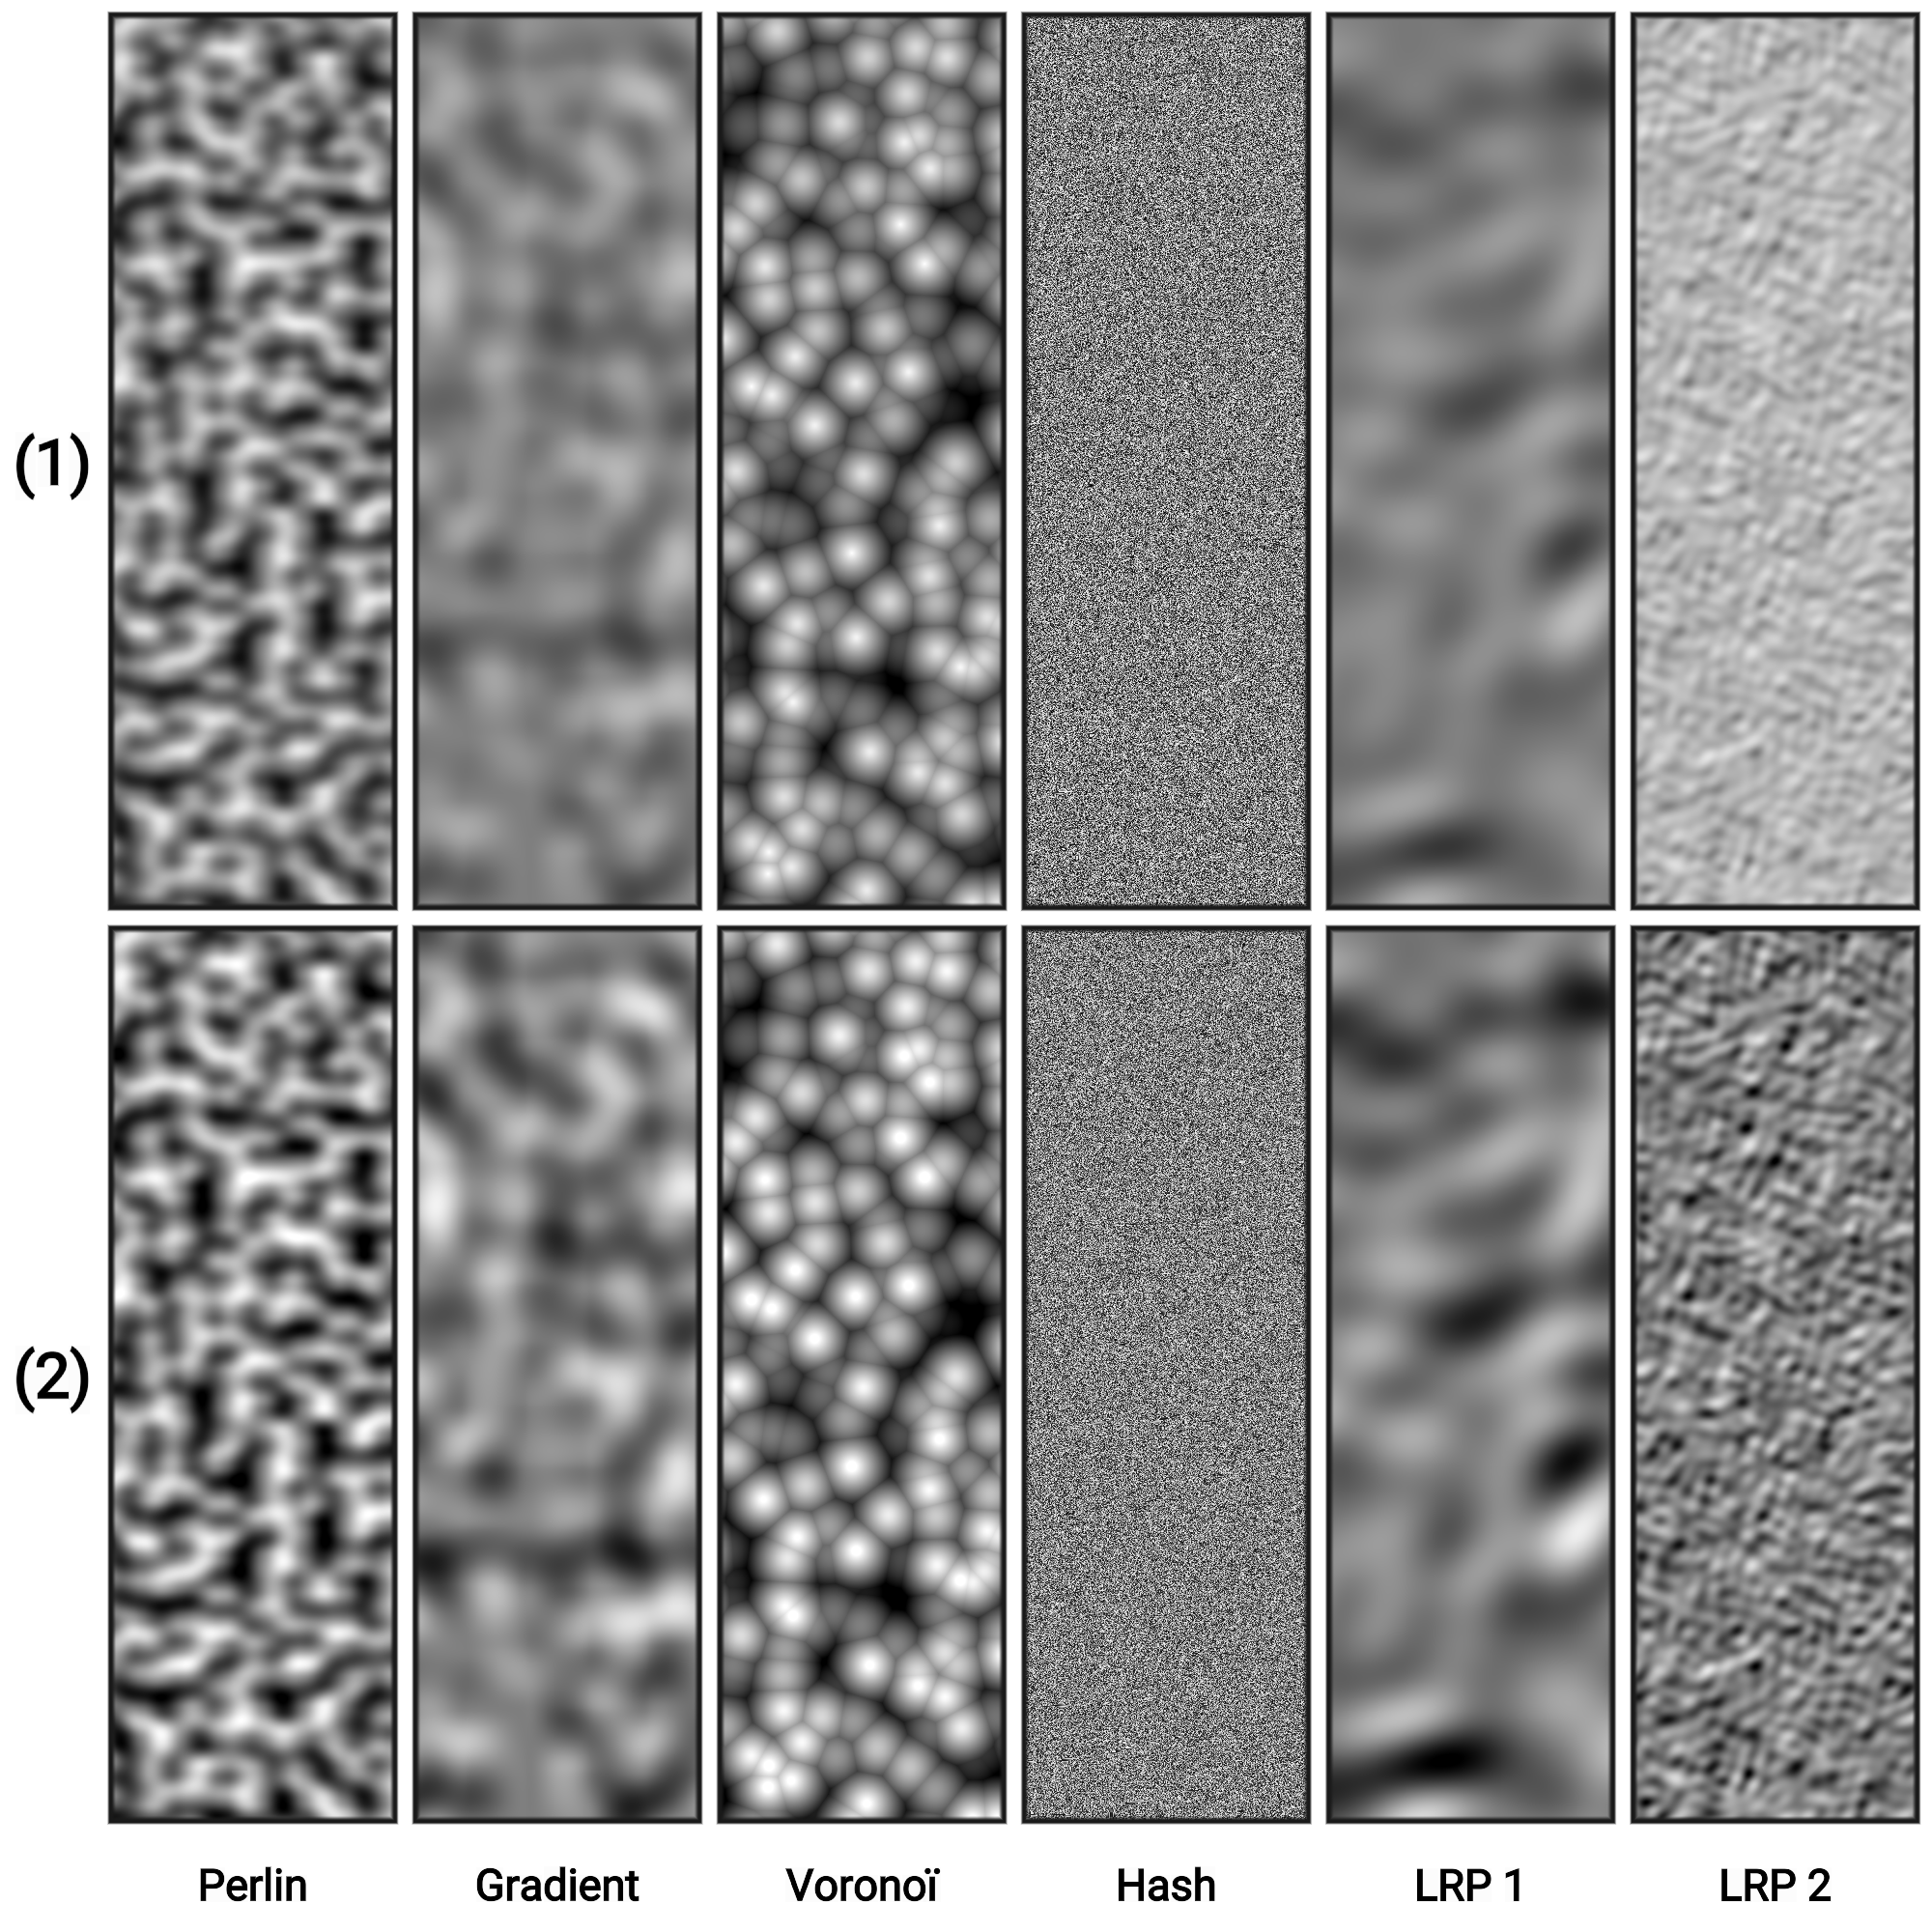
\includegraphics[width=\linewidth]{figures/MixMax_Priority.png}
  \caption{Comparaison entre les processus stochastiques originaux (1) et les résultats donnés par la fonction de priorité (2). Les niveaux de gris originaux (1) sont compris entre 0 (noir) et 1 (blanc) tandis qu'ils sont représentés la ligne (2) dans l'interval -1 (noir) à +1 (blanc).
  }
  \label{fig::MixMax_Priority}
\end{figure}

Nous proposons une solution, notée $\mathcal{P}$, de priorité procédurale
utilisant les propriétés statistiques d'un processus stochastique donné afin
d'en extraire une carte de priorité respectant l'intensité du bruit, le tout en
ayant une intensité correctement répartis entre $[-1, 1]$ pour n'importe quelle
entrée. Cette méthode s'apparente à l'approximation d'un étalement
d'histogramme utilisant l'espérance $\mathbb{E}$ et l'écart-type $\sigma$ d'une
variable aléatoire $V$.

\begin{equation}\label{ProceduralPriorityFormula}
  \mathcal P^{\pm 1}(V) =
  \pm
  \begin{cases}
    -1,                                         & \text{Si } V < \mathbb{E}[V]- \sqrt{\sigma[V]} \\
    +1,                                         & \text{Si } V > \mathbb{E}[V]+ \sqrt{\sigma[V]} \\
    \frac{V - \mathbb{E}[V]}{\sqrt{\sigma[V]}}, & \text{Sinon}
  \end{cases}
\end{equation}

Cette méthode donnera des bornes d'étalements, ie les bornes de l'interval
d'intensité dans l'entrée qui sera convertis à $[-1, 1]$ dans la sortie,
centrés sur $\mathbb{E}[V]$ et d'interval $2\sqrt{\sigma[V]}$.

\begin{equation}\label{PriorityBornes2}
  \begin{split}
    \lim_{V \rightarrow \mathbb{E}[V] - \sqrt{\sigma[V]}}\mathcal{P}(V) = -1
    \\
    \lim_{V \rightarrow \mathbb{E}[V] + \sqrt{\sigma[V]}}\mathcal{P}(V) = +1
  \end{split}
\end{equation}

Dans la figure \ref{fig::MixMax_Priority}, nous observons que la correction de
contraste obtenue avec cette méthode est équilibré sur tous les processus que
nous avons pus tester.

\begin{figure}
  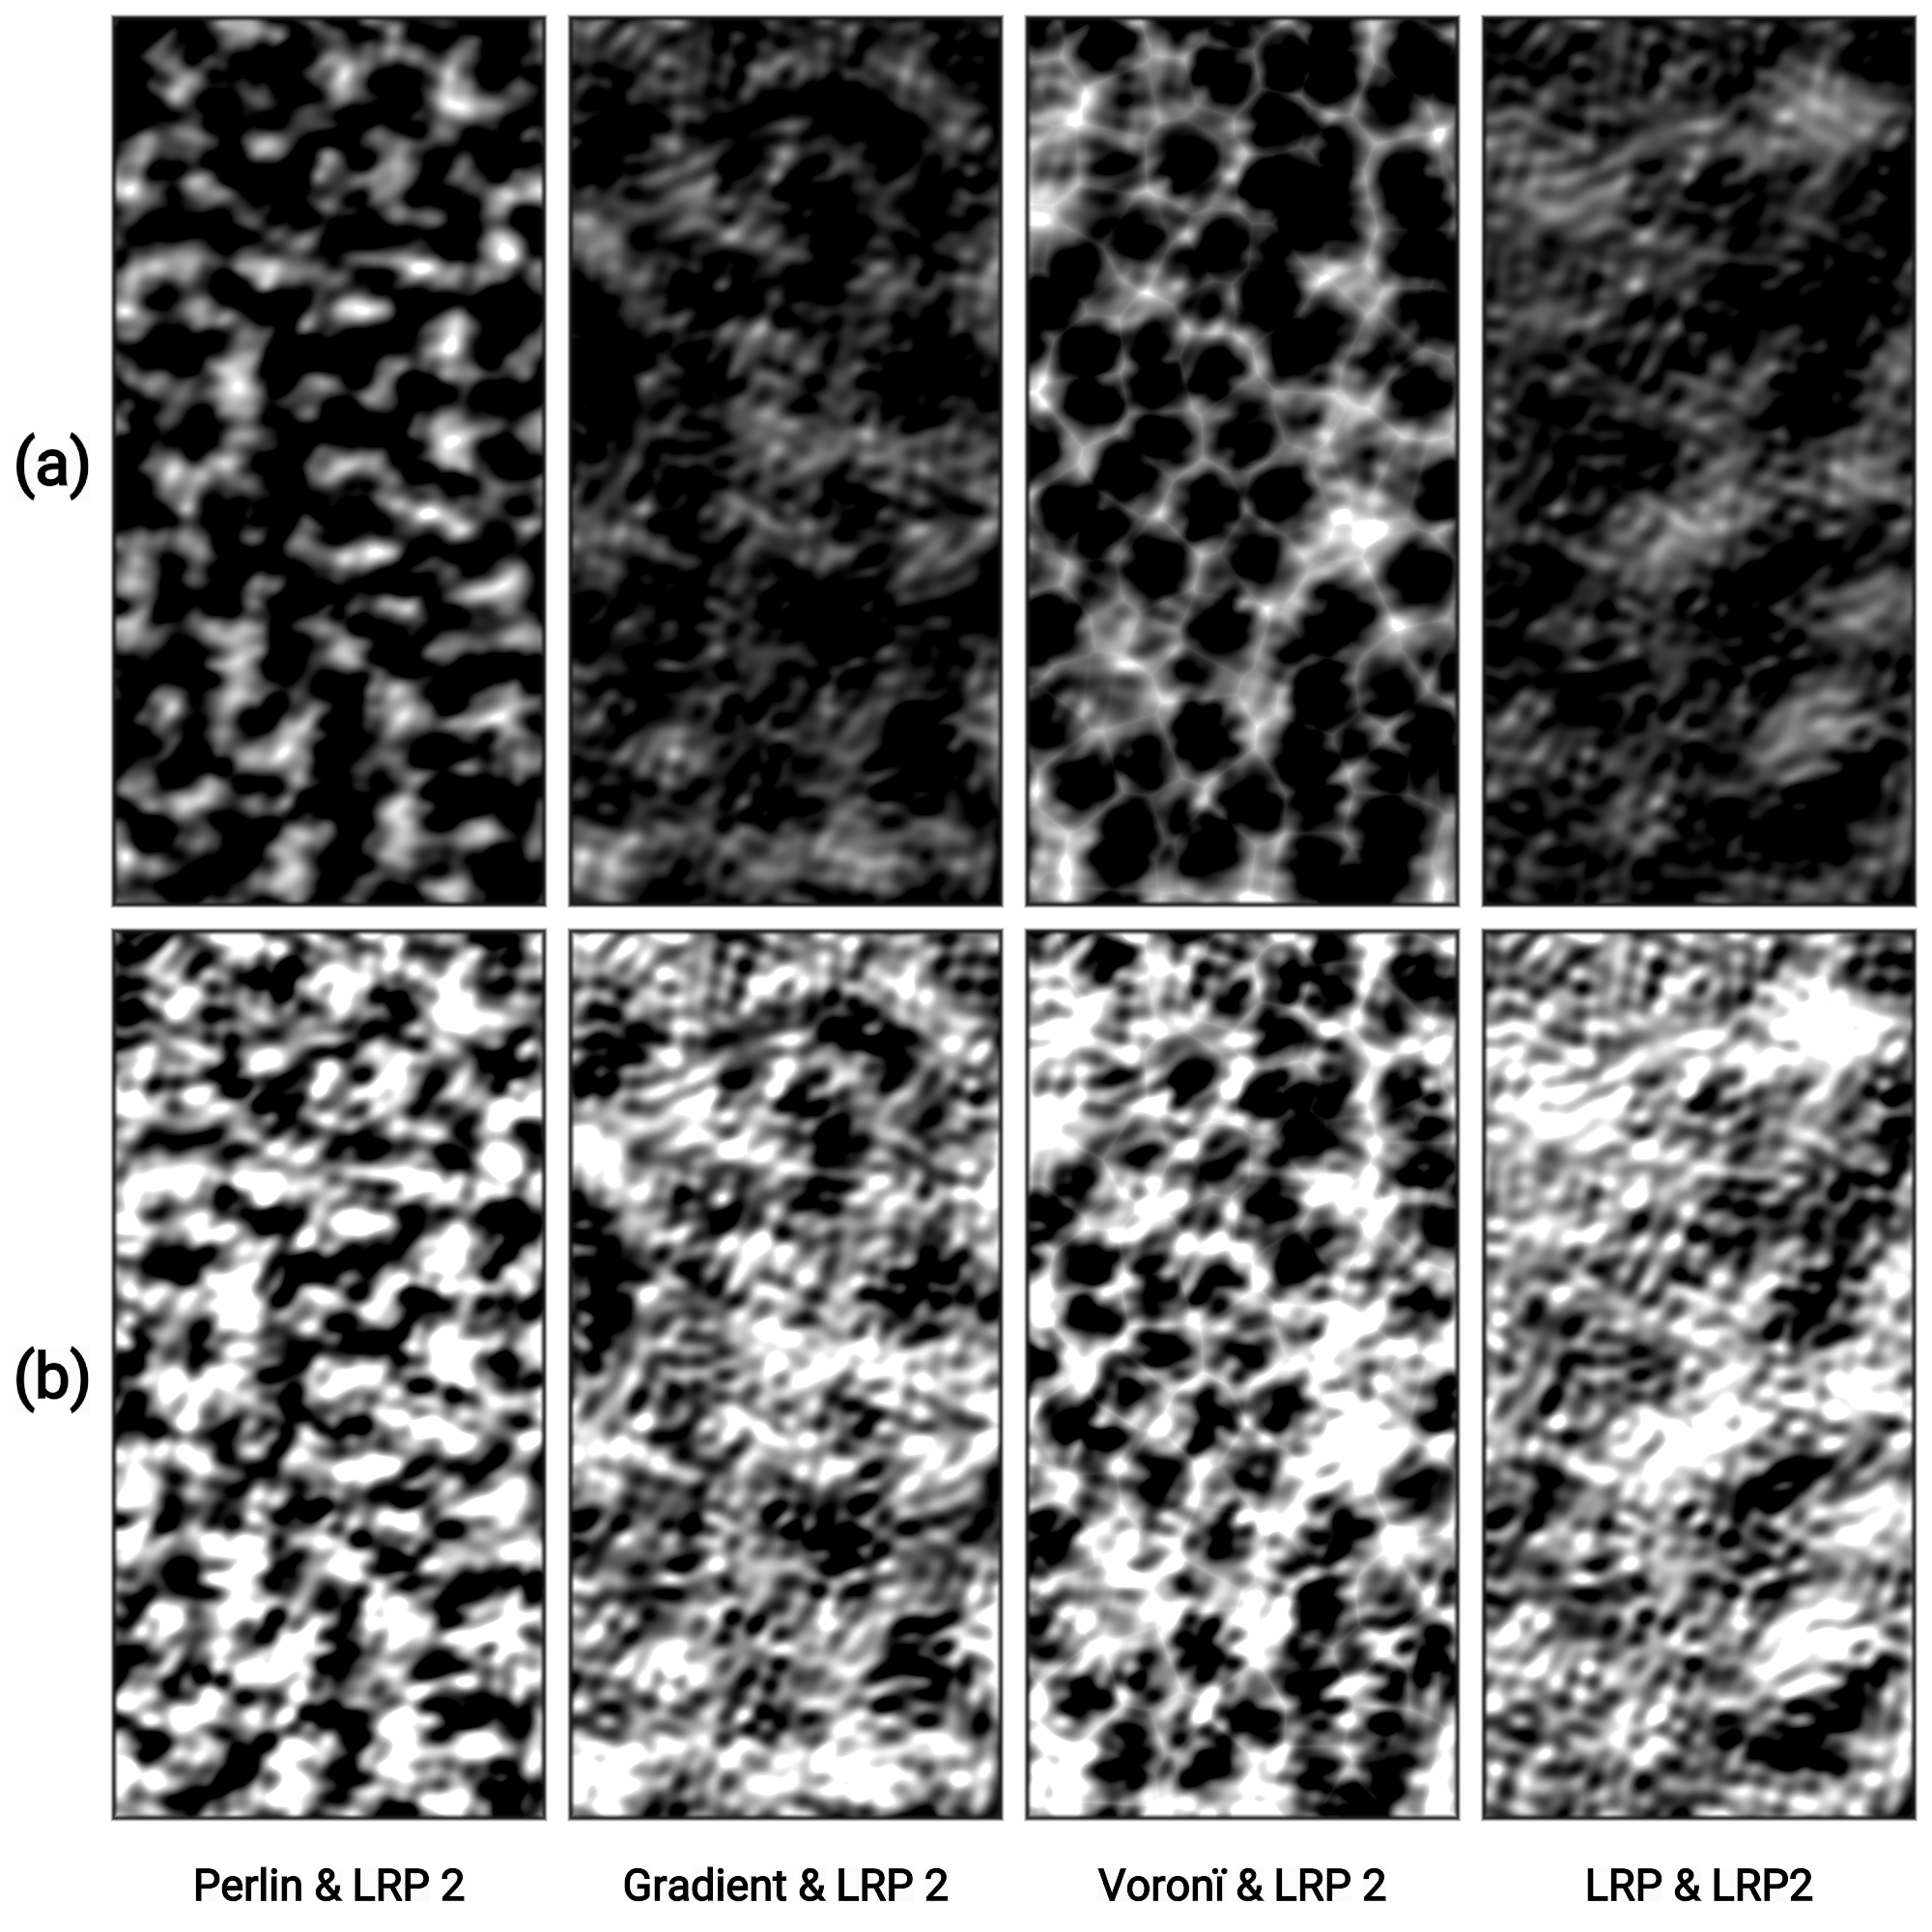
\includegraphics[width=\linewidth]{figures/MixMax_PriorityCorrection.png}
  \caption{
    Résultats de notre fonction d'influence avec un biais d'entrée de 0.5 sans correction de la priorité (a) et après réhaussement de la priorité (b). Nous observons à la ligne (b) une fréquence de présence similaires entre les processus, peut importe leur propriétés statistiques.
  }
  \label{fig::MixMax_PriorityCorrection}
\end{figure}

\subsection{Nouvel opérateur d'influence équilibré}

Nous proposons un opérateur d'influence $\mathcal{A}$ entre deux processus
stochastiques $V_0$ et $V_1$ basé sur les principes du MixMax, simplifiant la
formule donnée dans le papier original \cite{mixmax} grâce aux propriétés
obtenues par notre fonction de priorité procédurale.

\begin{figure}
  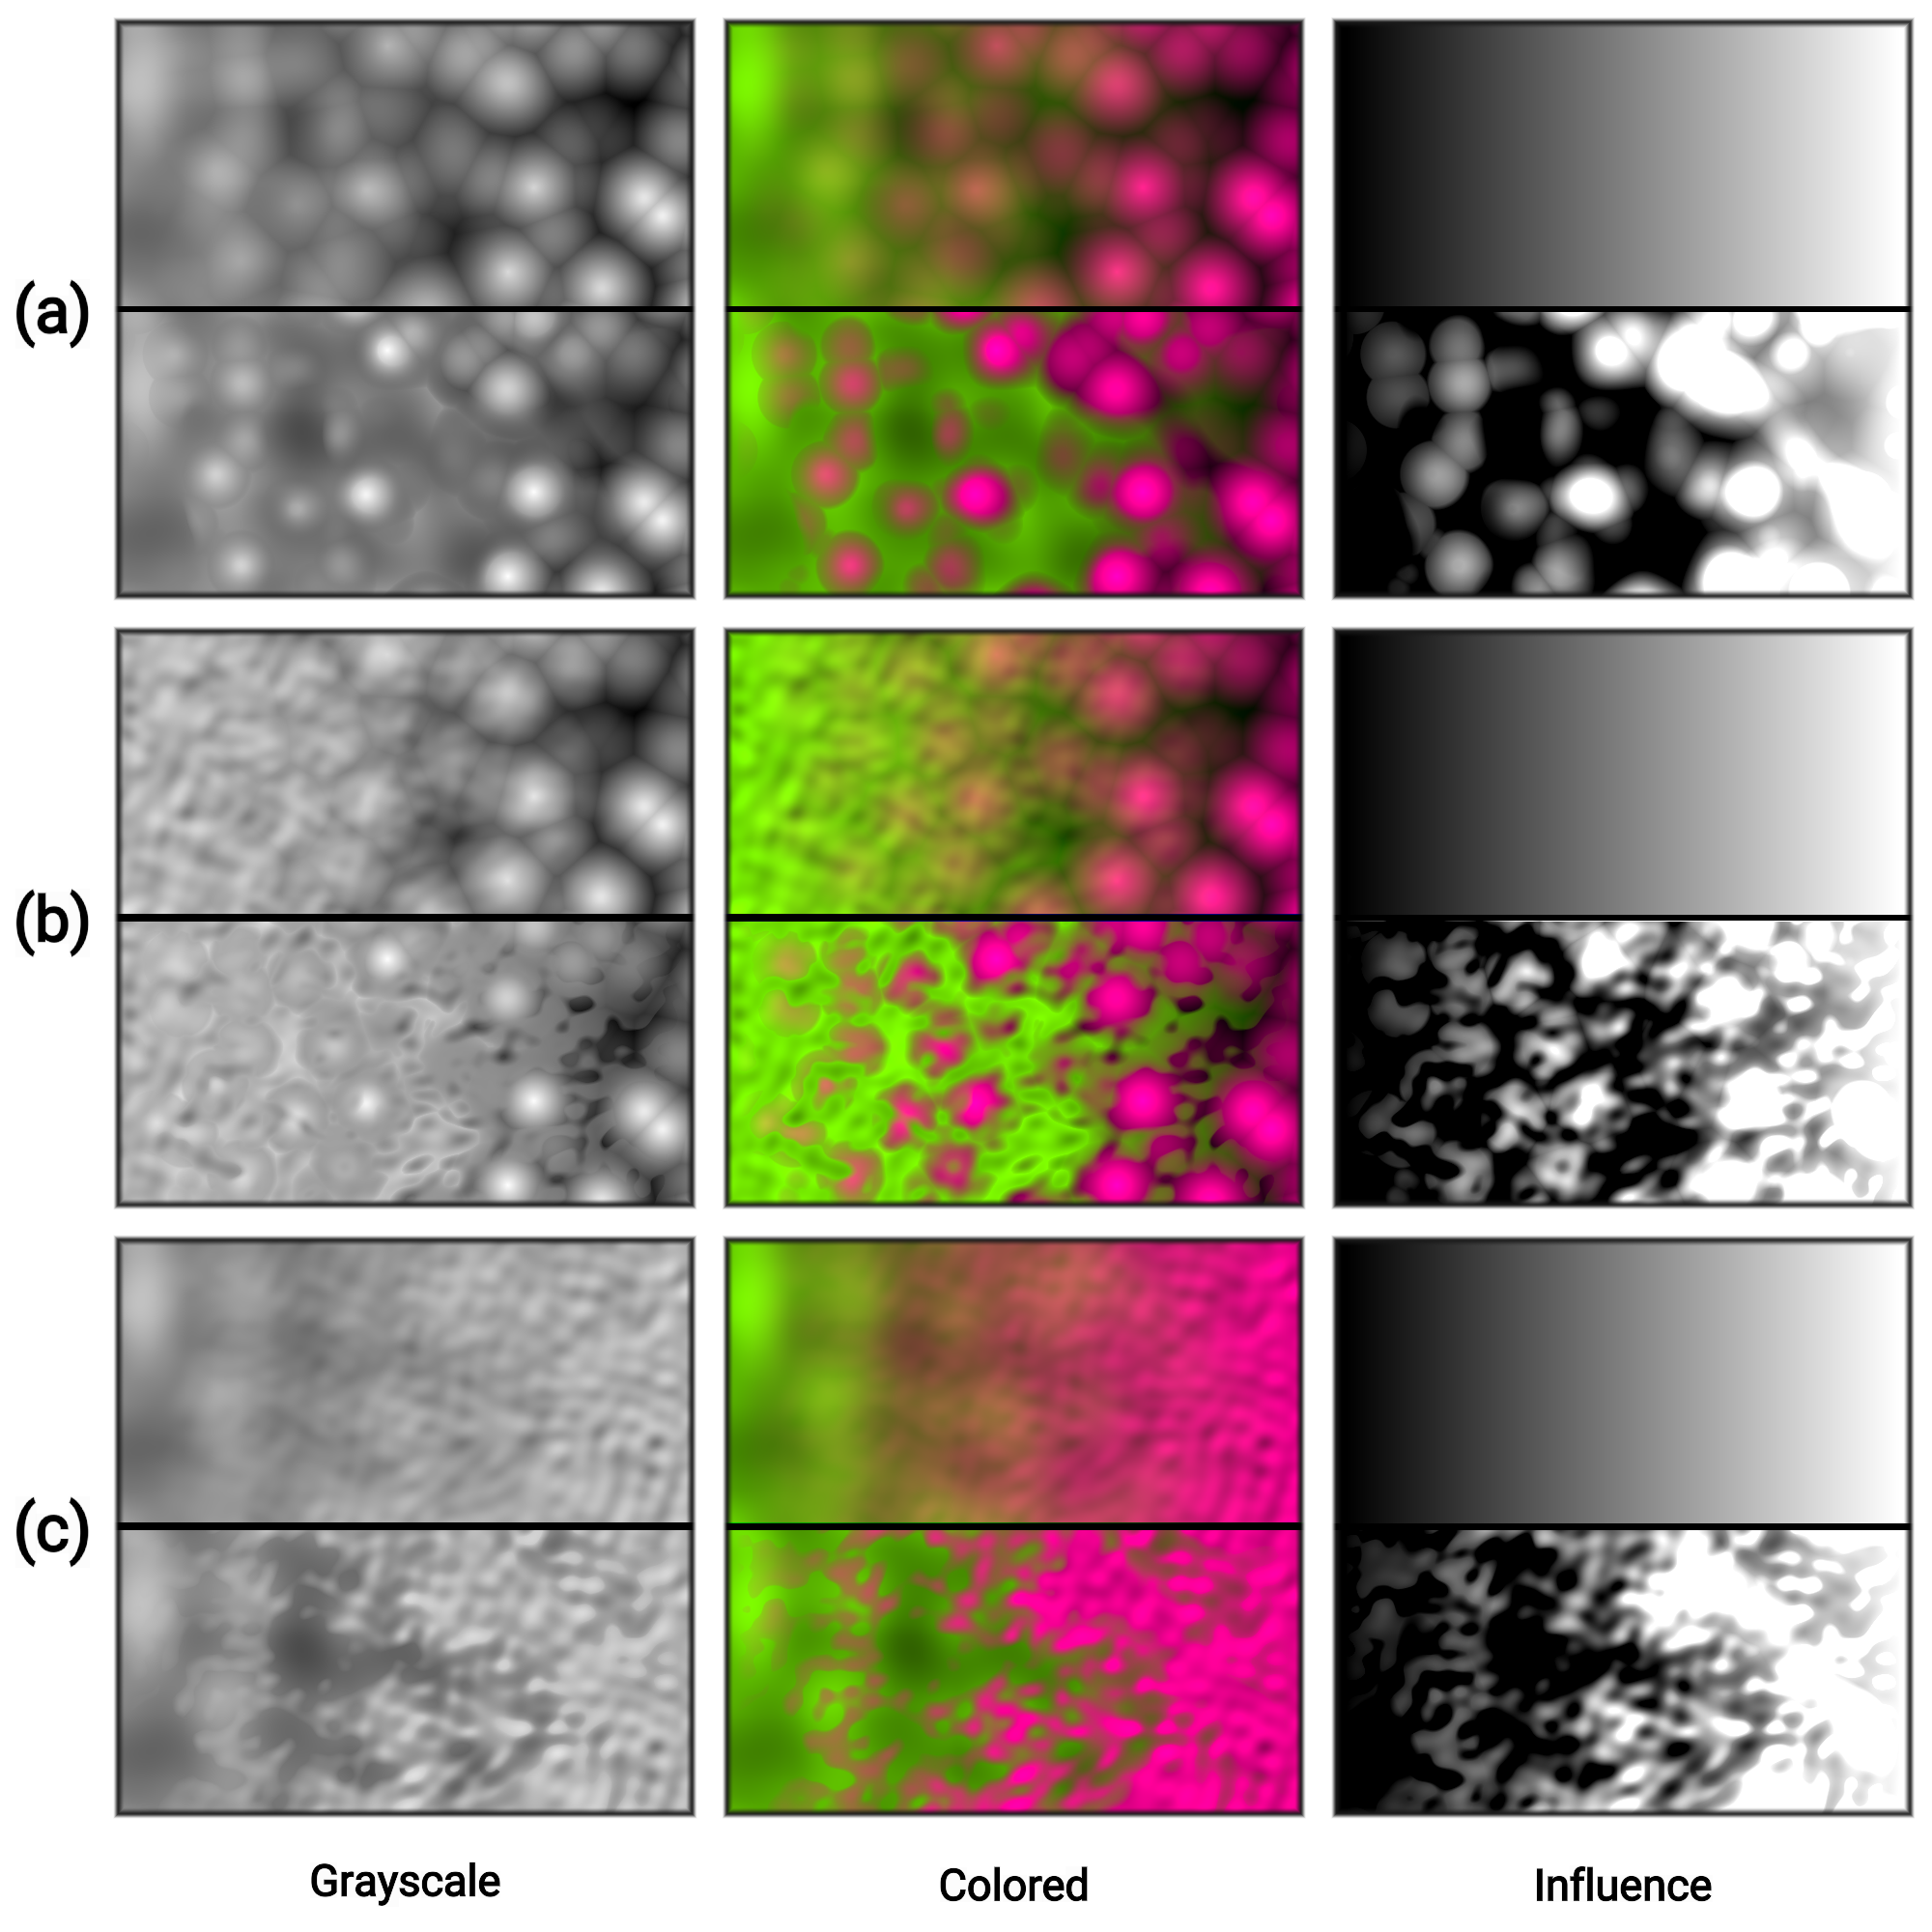
\includegraphics[width=\linewidth]{figures/MixMax_Comparaison.png}
  \caption{
  Résultats du mélange entre Voronoï et Gradient (a), Voronoï et LRP2 (b) ainsi que LRP2 et Gradient (c). La moitié supérieur des céllules montrent un gradient d'influence linéaire $\alpha$ et la partie inférieur un gradient utilisant la fonction $\mathcal{A}^c_{0.5}$ en influence.}
  \label{fig::MixMax_Comparaison}
\end{figure}

% \begin{equation}
%   \begin{split}
%     \mathcal S^b_a(x) &=
%     \begin{cases}
%       0,                                                                      & \text{Si } x < a \\
%       1,                                                                      & \text{Si } x > b \\
%       3\left(\frac{x - a}{b - a}\right)^2-2\left(\frac{x - a}{b - a}\right)^3 & \text{Sinon}
%     \end{cases}
%     \\
%     \\
%     \mathcal{A}^r_s(V_0, V_1, \alpha)  &= \mathcal S^{+s}_{-s}\left(
%     \frac{\mathcal P^{\pm 1}(V_0) +\mathcal P^{\pm 1}(V_1)}{2}+ \alpha\left(s + \frac{1}{r}\right)\right)
%   \end{split}
% \end{equation}

\begin{equation}\label{A_base}
  \begin{split}
    \mathcal L_a(x) &=
    \begin{cases}
      0,                        & \text{Si } x < a \\
      1,                        & \text{Si } x > b \\
      \frac{x}{a} - \frac{1}{2} & \text{Sinon}
    \end{cases}
    \\
    \\
    \rho &= \frac{\mathcal{P}^{\pm 1}_{V_0} + \mathcal{P}^{\pm 1}_{V_1}}{2}
    \\
    \\
    |\rho| &= \frac{|\mathcal{P}_{V_0}| + |\mathcal{P}_{V_1}|}{2}
    \\
    \\
    \mathcal{A}_s &= \mathcal{L}^s\left(
    \rho + (2 \alpha - 1)(s + |\rho|)
    \right)
  \end{split}
\end{equation}

Cette fonction utilise un biais linéaire $\alpha$ ainsi qu'une valeur de
lissage $s$ strictement positive. Nous montrons l'impact de ces paramètres sur
le mélange dans la figure \ref{fig::MixMax_SmoothnessAlpha}.

Chacune des deux fonction de priorité peut être inversée. Les différences
visuelles qu'impliquent ces inversions sont visibles sur la figure
\ref{fig::MixMax_Invert}, où l'équilibre du constrast dans les zones de
transition varie en fonction du paramétrage.

Lorsque nous comparons la moyenne des présences de chaque bruit en fonction de
$\alpha$, nous remarquons des imrpécésions. L'influence de sortie suit une
transition douce lorsque l'écart des priortés à la moyenne est grand. Le
principe de transition douce est un outil régulièrement utilisé dans la
création de mouvements ou de transitions agréables à l'oeil humain. Cependant,
ce phénomène entraine une disparité de présence des bruits dans notre mélange.
Nous proposons une version corrigée de notre méthode prennant en compte ce
biais et le corrigeant à l'aide de la fonction de transition douce inverse
$\mathcal{S}^{-1}$ :

\begin{figure}
  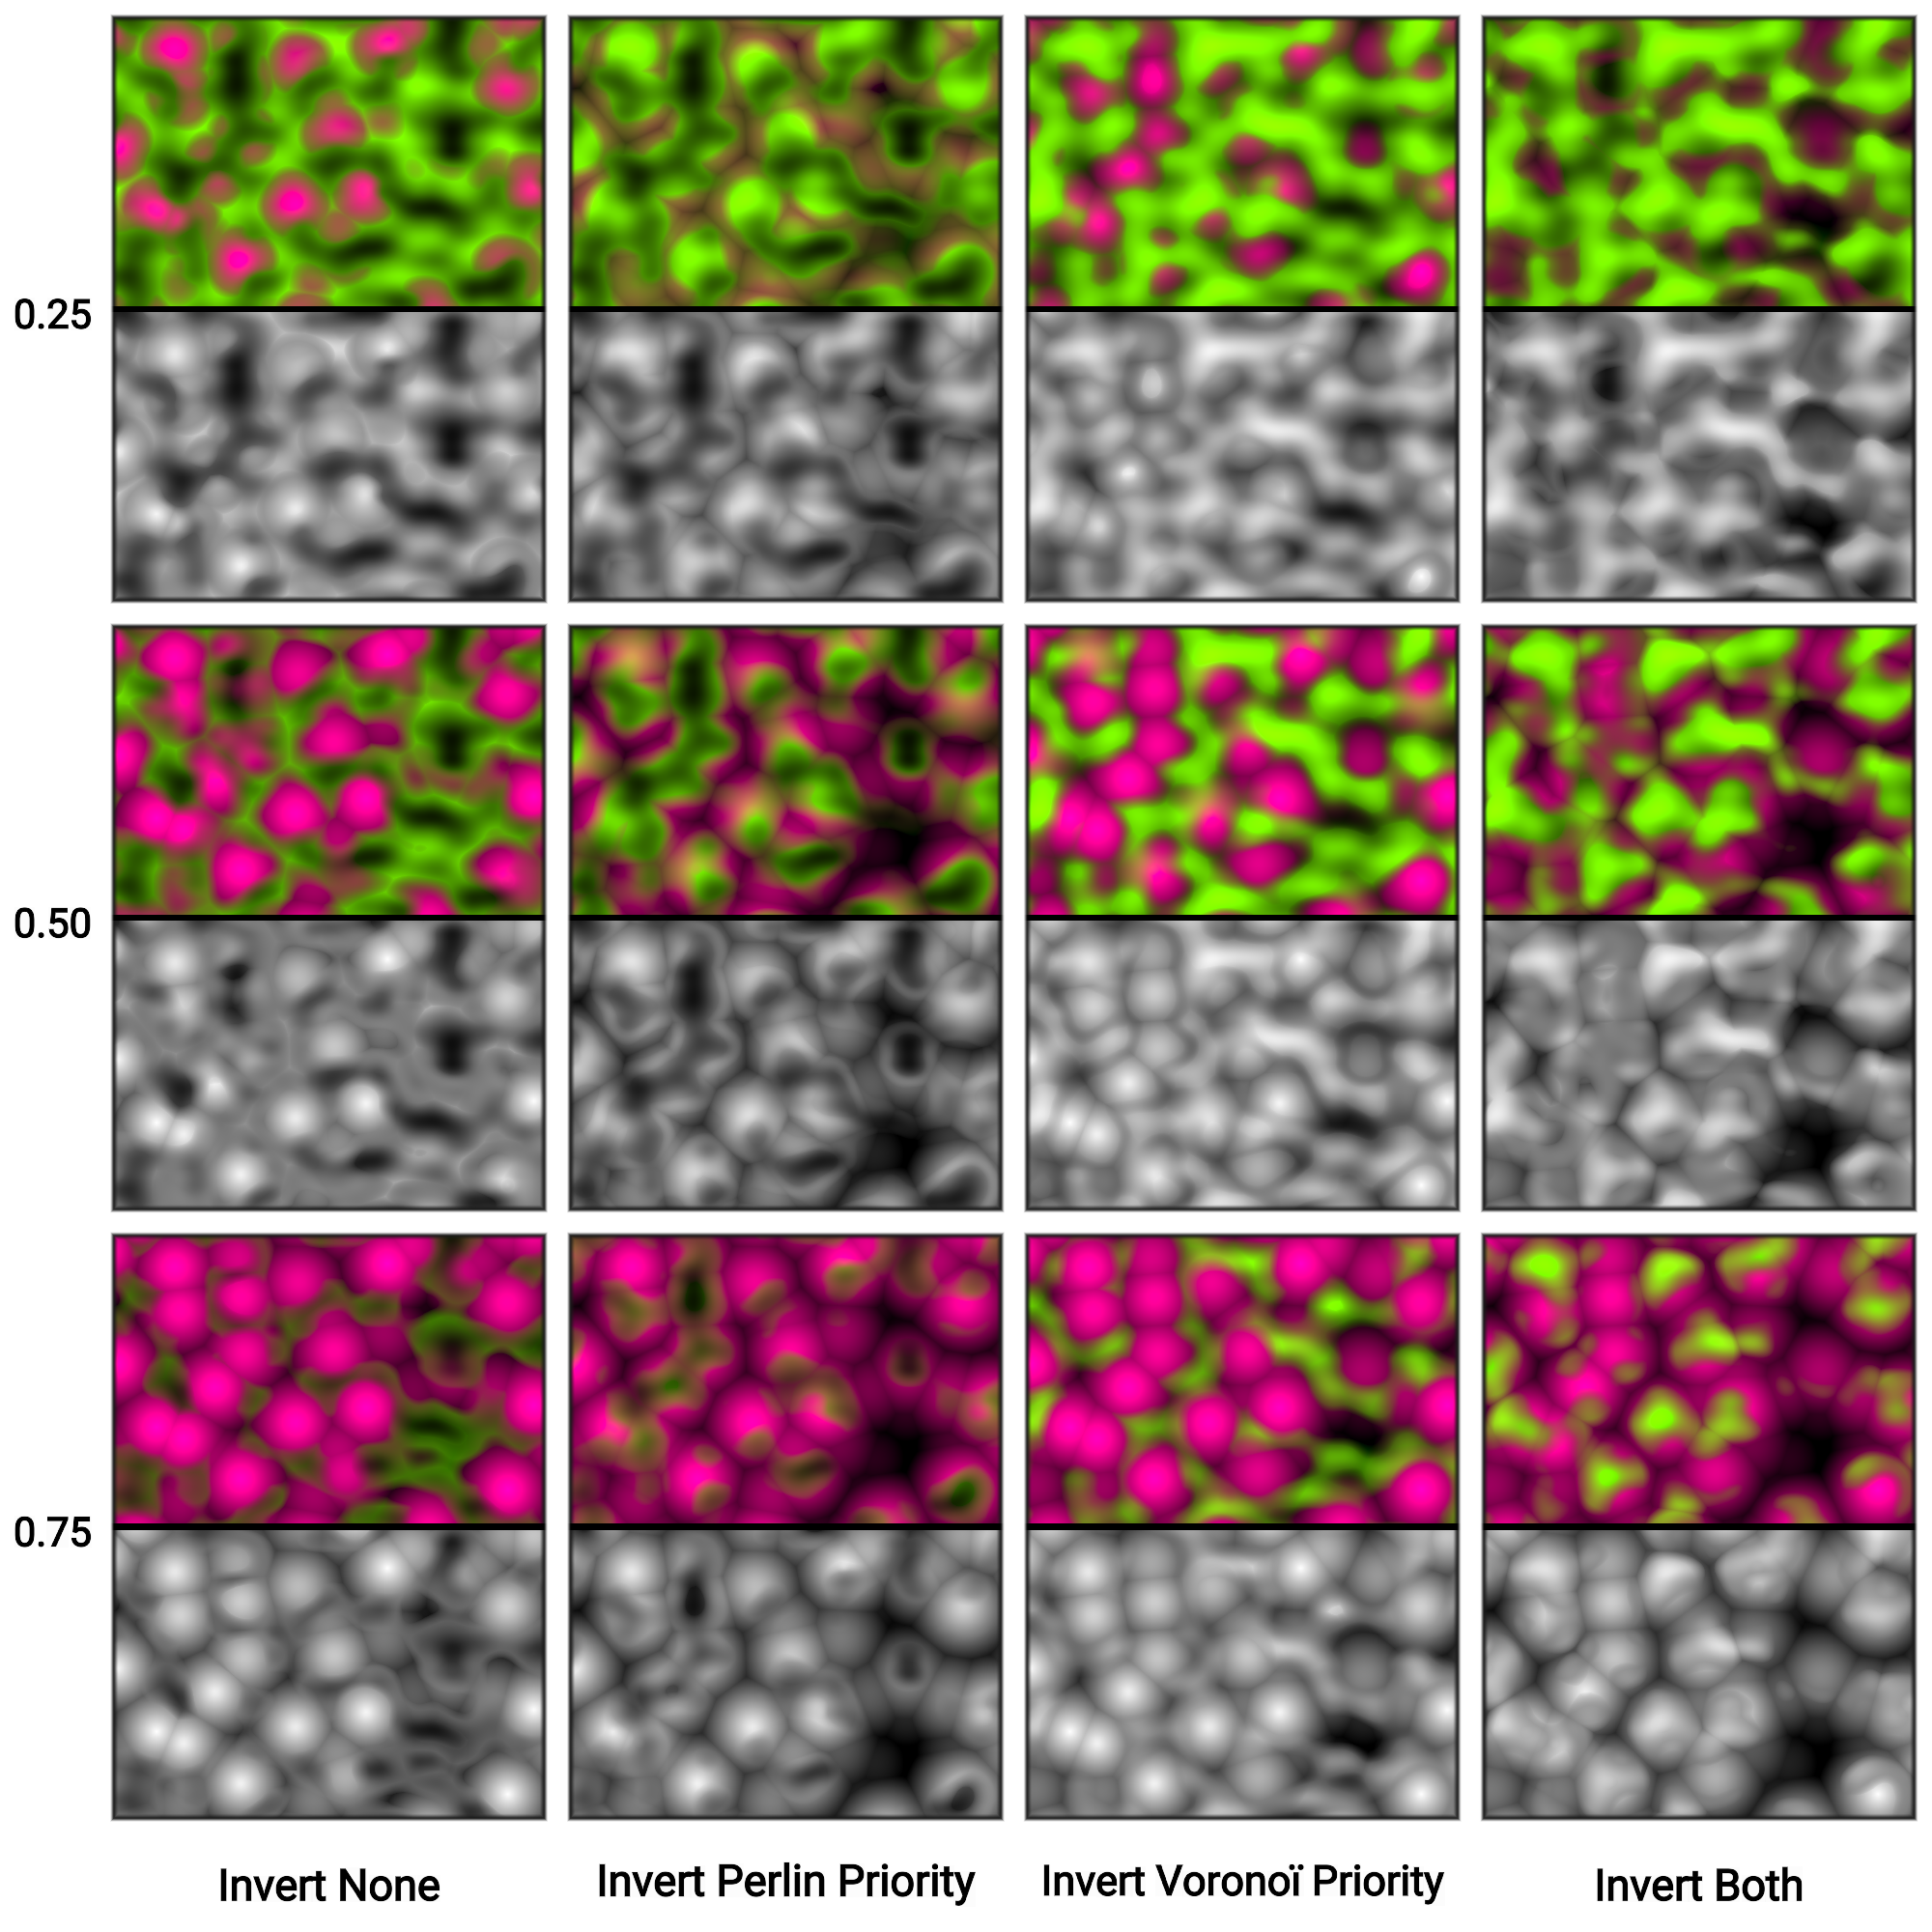
\includegraphics[width=\linewidth]{figures/MixMax_Invert.png}
  \caption{
  Résultats du mélange utilisant $\mathcal{A}^c_{0.5}$ entre Voronoï et Perlin en fonction du biais d'entrée $\alpha$ (lignes) et des directives d'inversions de priorités (colonnes). Nous remarquons que lorsqu'une seule des priorité est inversée, des biais statistiques deviennent visibles.
  }
  \label{fig::MixMax_Invert}
\end{figure}

\begin{equation}\label{A_corrected}
  \mathcal{A}_s^c =
  |\rho| \mathcal{S}^{-1}(\mathcal{A}_s)
  +
  (1-|\rho|)\mathcal{A}_s
\end{equation}

% Pour finir, l'utilisation de la fonction $\mathcal{S}$, dite de transition
% douce, permet d'obtenir de meilleur transitions entre les entrées. Cette
% fonction représente une transition non linéaire entre deux valeurs respectant
% le principe d'atténuation en sortie et en entrée. Ce principe est régulièrement
% utilisé dans l'animation ou la création de transitions visuelles. Cette
% fonction peut être remplacée par n'importe quel autre polynôme respectant les
% propriétés d'une transition. Cependant, dans notre MixMax, nous utiliseront la
% fonction $\mathcal{S}$ pour sa pertinence dans la création de transition
% nettes.

\newpage

\begin{figure}
  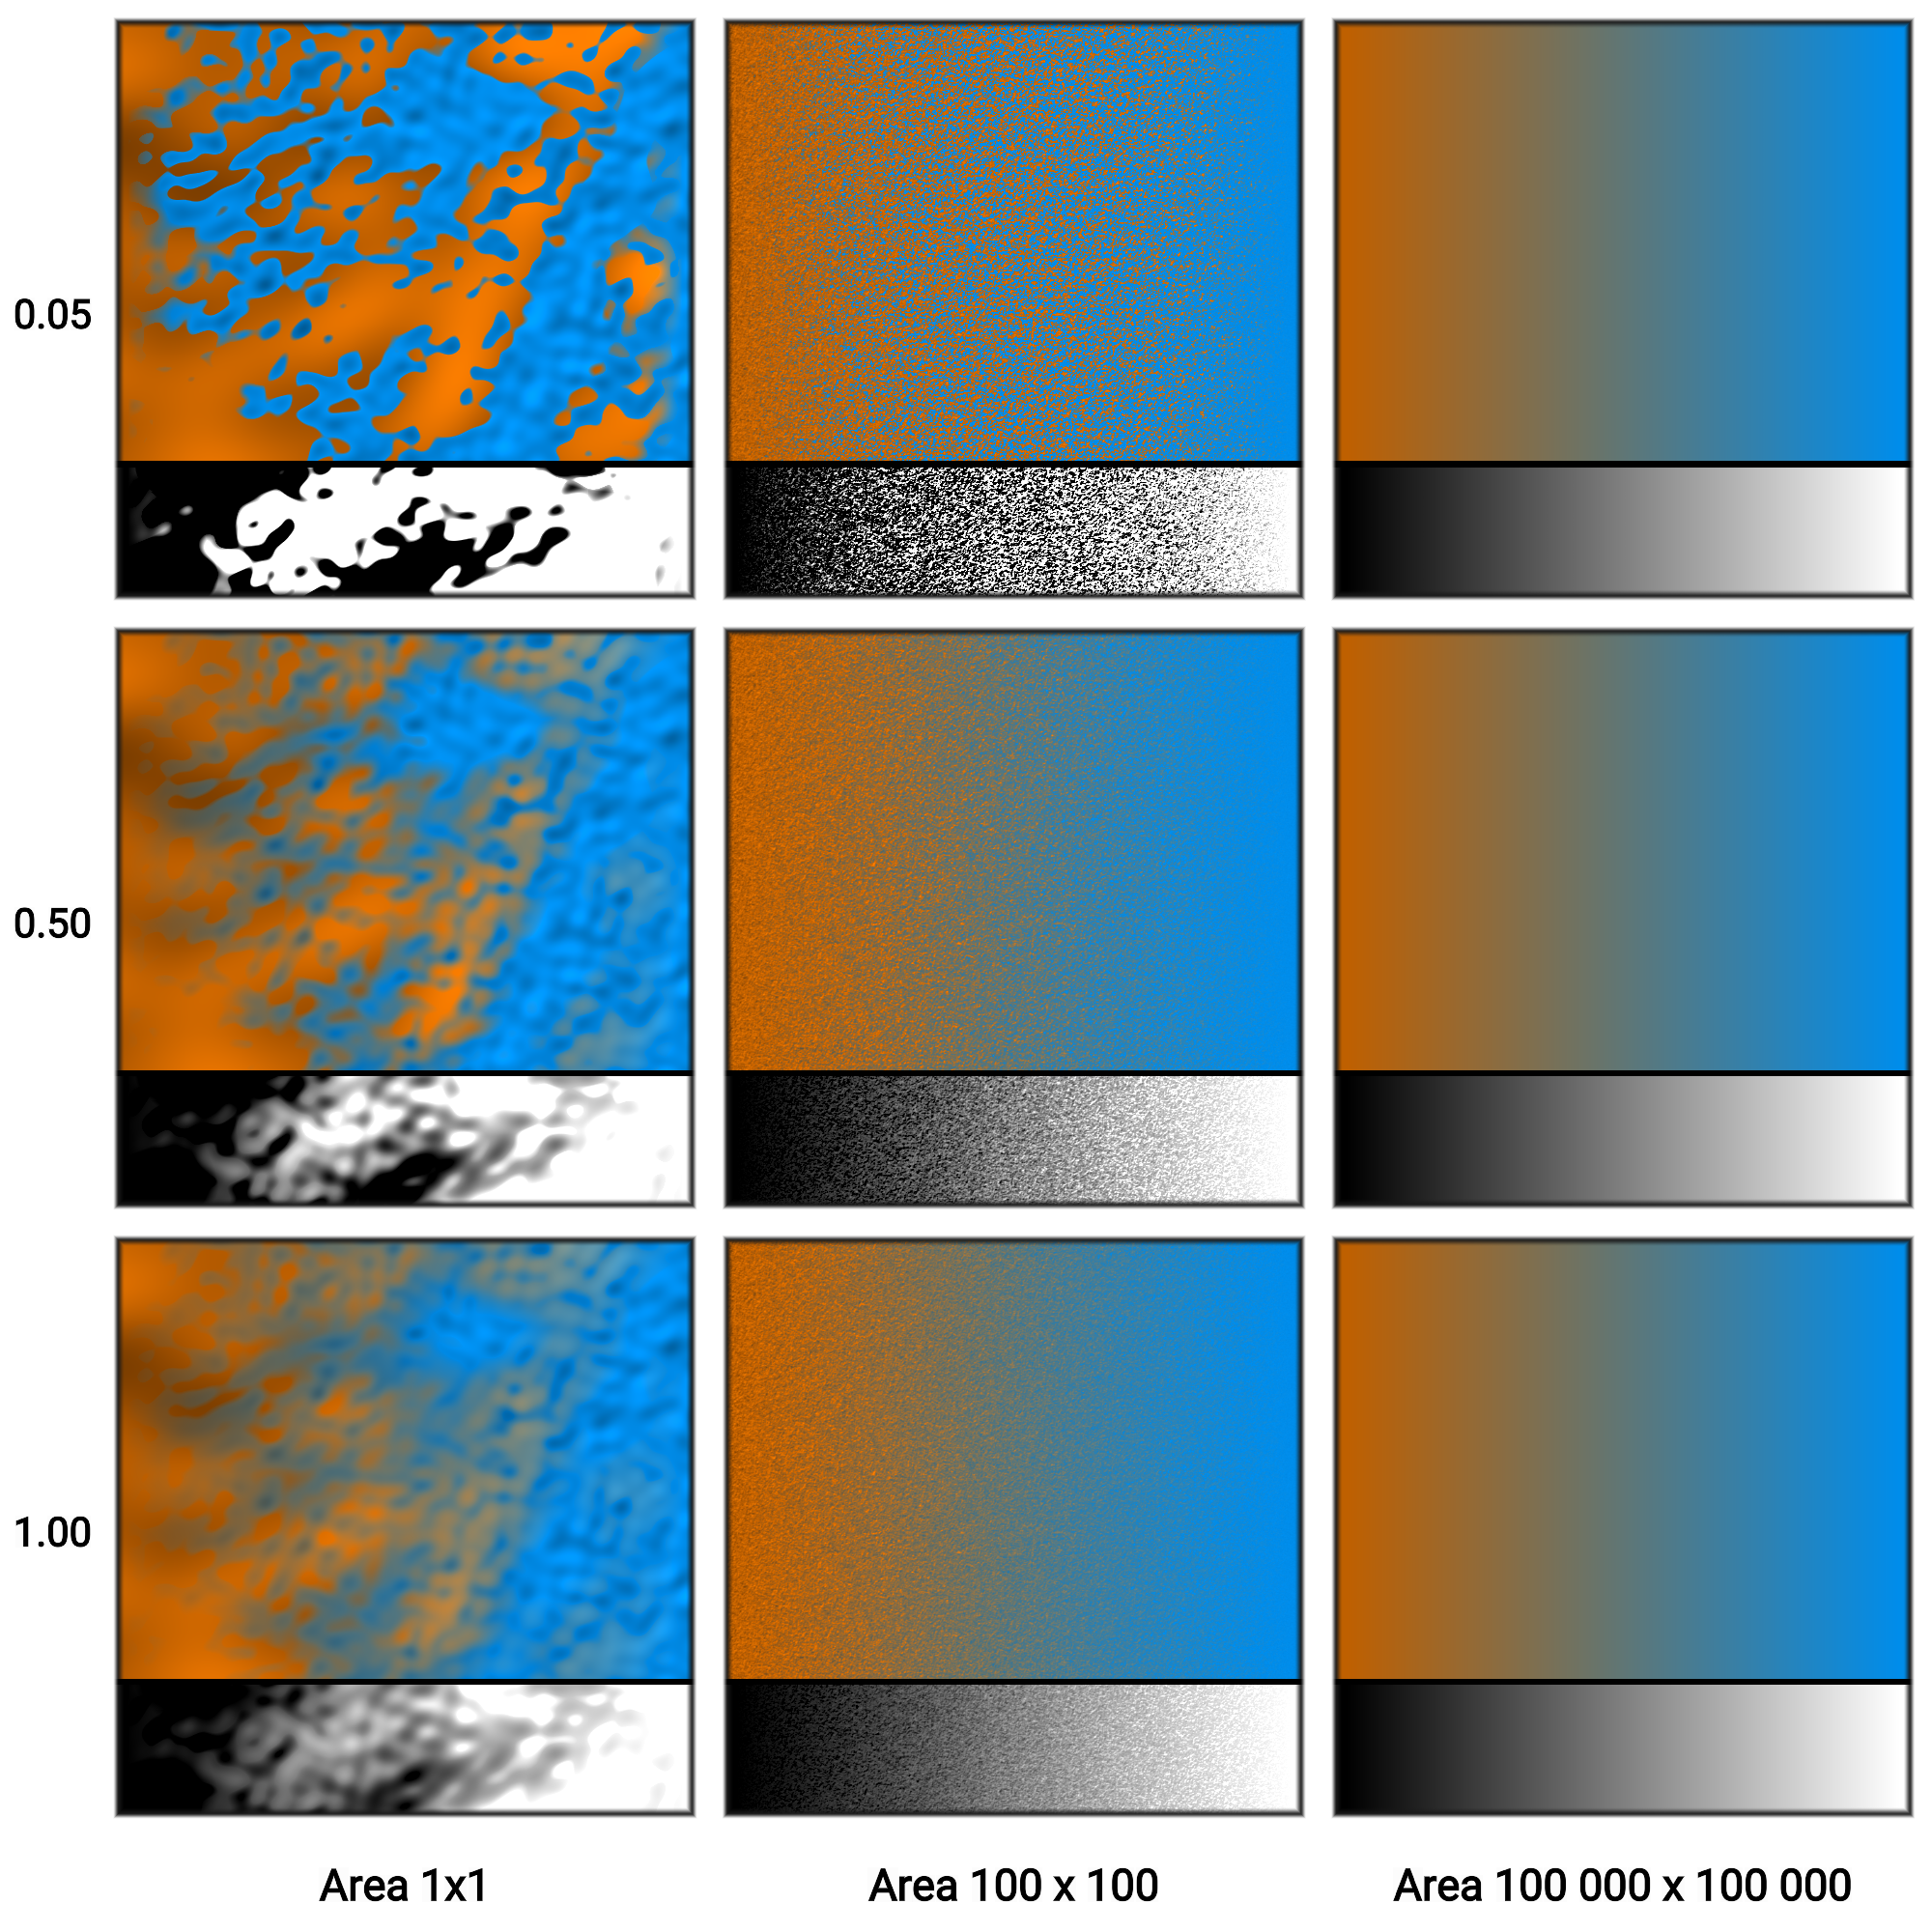
\includegraphics[width=\linewidth]{figures/MixMax_Scale.png}
  \caption{
    Résultats de transition utilisant $\mathcal{A}^c_s$ entre deux processus analytiquement filtrable LRP1 et LRP2 en fonction du lissage $s$ (lignes) et de la taille de la zone $\mathbb{P}$. Les entrées du mélange sont colorés pour une meilleur visibilité. La valeur de l'influence est également visible dans le quart inférieur de chaque céllule.
  }
  \label{fig::MixMax_Scale}
\end{figure}

\subsection{Démonstration de l'intégration}

Comme expliqué dans la section 1.2.6, le rendu d'une surface en temps réel
nécéssite un filtrage analytique de sa texture. Dans notre cas, nous notons
$V(\mathbb{P})$ l'empreinte d'une variable aléatoire $V$ sur la zone
$\mathbb{P}$ de taille $||\mathbb{P}||$. Selon l'équation \ref{A_base}, nous
obtenons :

% Faire : L'espérence, selon la réalisation, de l'influence lorsque la zone tend vers 0 est égal à...

\begin{equation}\label{A_filtrage_limites}
  \begin{split}
    \lim_{||\mathbb{P}|| \rightarrow +\infty} \mathcal{P}_{V}(\mathbb{P}) &= 0
    \\
    \lim_{||\mathbb{P}|| \rightarrow +\infty} \mathcal{A}_s^c(\mathbb{P}) &= \alpha(\mathbb{P})
    \\
    \lim_{||\mathbb{P}|| \rightarrow +\infty} \mathcal{A}_s(\mathbb{P}) &= \alpha(\mathbb{P})
  \end{split}
\end{equation}

Sur les très larges zones, notre mélange est ainsi correctement filtré
analytiquement. Cependant, comme vu précedement, sur des petites zones,
l'espérance de la présence des entrées n'est pas linéaire avec $A_s$. La
correction $A_s^c$ permet ainsi d'obtenir un filtrage très précis.

\begin{equation}\label{A_filtrage_limites2}
  \begin{split}
    \int_{\omega} \lim_{||\mathbb{P}|| \rightarrow 0} \mathcal{A}_s(\mathbb{P}) &\approx \mathcal{S}(\alpha(\mathbb{P}))
    \\
    \int_{\omega} \lim_{||\mathbb{P}|| \rightarrow 0} \mathcal{A}_s^c(\mathbb{P}) &\approx \alpha(\mathbb{P})
  \end{split}
\end{equation}

Lorsque la valeur de lissage $s$ est très petite ($s < 0.05$), l'écart de cette
approximation avec le filtrage réel s'accroie. Cependant, nous n'avons pas
trouvé de marge d'érreure significative dans notre implémentation pour toutes
les valeurs de $s$ supérieurs à 0.05.

\begin{figure}
  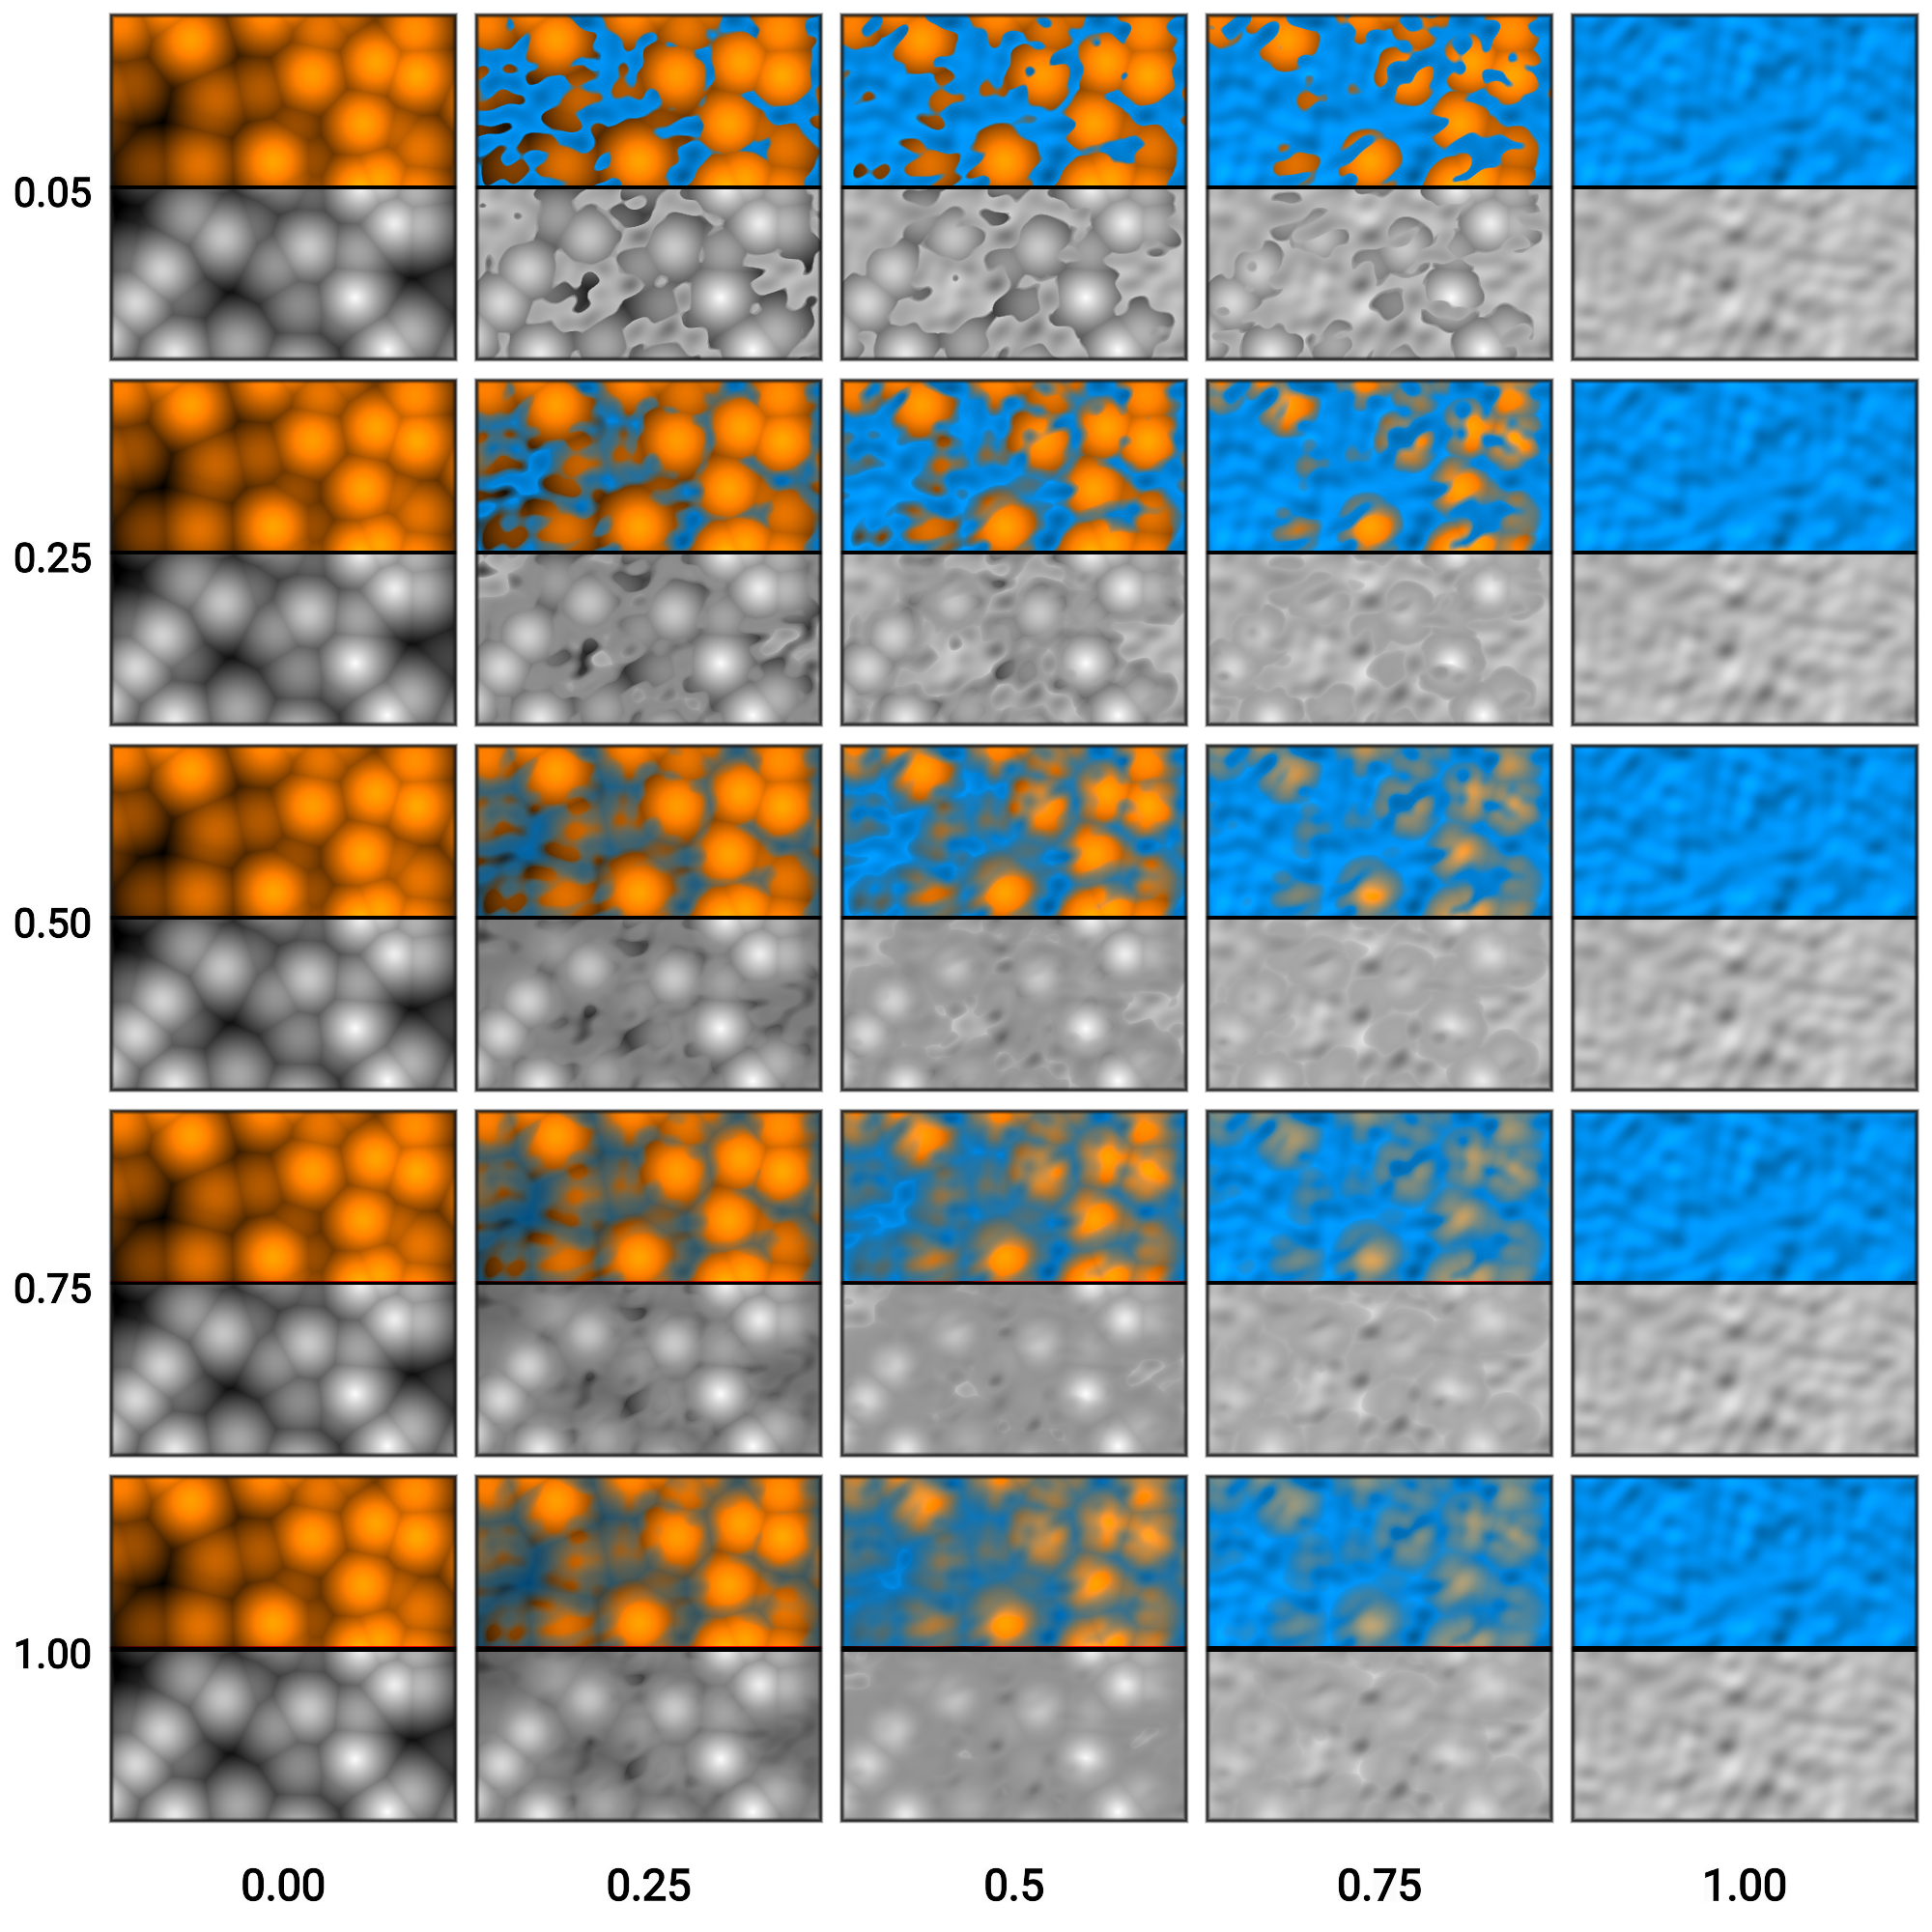
\includegraphics[width=\linewidth]{figures/MixMax_Smoothness_Alpha.png}
  \caption{
    Résultats du mélange entre Voronoï et LRP2 utilisant $\mathcal{A}^c_s$ en
    fonction de $s$ (lignes) et du biais linéaire d'entrée $\alpha$ (colonnes). Les
    priorités des deux entrées sont inversées.
  }
  \label{fig::MixMax_SmoothnessAlpha}
\end{figure}

\subsection{Conclusion}

La méthode que nous proposons permet de créer des transitions nettes et
sensibles au contenu entre n'importe quel processus stochastique. La formule
utilisé est analytiquement filtrable lorsque toutes les entrées le sont
également. Cependant, certaines limitations persistent, comme les imrpécésions
de filtrage pour des transitions très nettes.

Un tel outil ouvre un large champ de possibilités pour la création de processus
stochastiques à variation spatialle, le tout en temps réel et avec un très
faible impact en calcul et en mémoire.

\clearpage

\printbibliography %Prints bibliography

\end{document} % This is the end of the document
